\chapter{Methods: Example Application and Library}
\label{chapter:methods}

\section{Qt Developer Days 2011 Conference Schedule Application}
\label{section:devdays}

\section{JSONCache JavaScript Library}
\label{section:jsoncache}

JSONCache is a lightweight JavaScript library for fetching \abbr{JSON}
data in flaky networks. The library was designed especially to handle
flaky mobile networks with connection problems and short
interruptions. The goal is to avoid networking as long as possible and
failing gracefully if network connections are not stable.

JSONCache provides two main functionalities: data caching and
attempting to fetch the data multiple times.

The caching layer uses the client side localStorage \citationneeded
cache of \abbr{HTML5}. Data requests can be done using the JSONCache
\abbr{API} which always checks the local cache first before opening
any network connections. If the data is already in the cache, the
cached data is checked for validity and if the data has not been
expired, it is returned immediately. If the data is not in the cache
or it has been expired, a new network request is made and the received
data is cached and returned to the requestor. The expiration time of a
data item can be configured in the library settings.

JSONCache also tries to fetch the data multiple times to handle small
interruptions in network connection. \fixme{add example and explain
  that it is very common}. If a data fetch fails, a new fetch is
issued after a timeout (defined in the configuration). On subsequent
attempts the timeout is increased, and after a defined number of
attempts the fetch error is issued to the requestor.

Figure~\ref{figure:jsoncache-demo.png} shows an interactive demo of
the JSONCache library. The
demo\footnote{\url{http://kpuputti.github.com/JSONCache/demo/index.html}}
simulates the caching and fetching functionality of the library by
simulating a flaky network according to the configuration.

\begin{figure}[ht]
  \begin{center}
    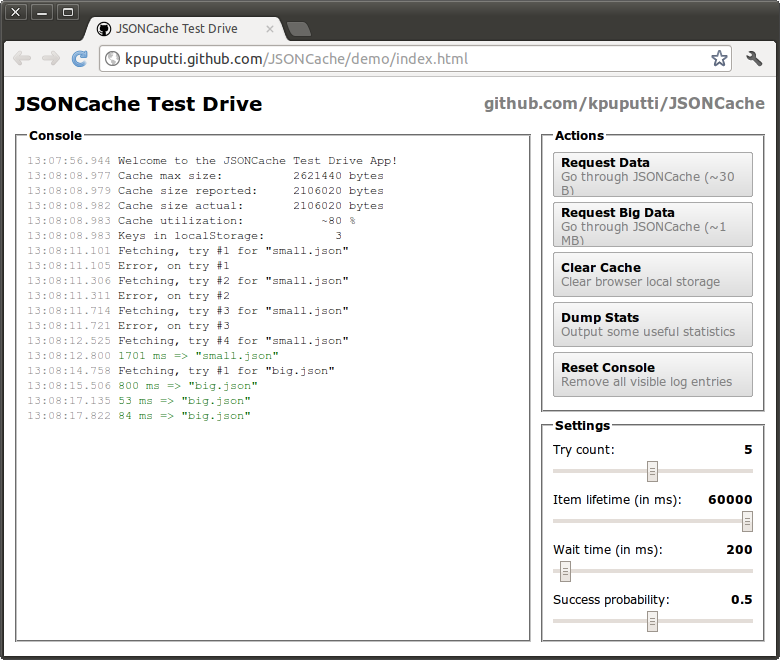
\includegraphics[width=\textwidth]{images/jsoncache-demo.png}
    \caption{Interactive JSONCache demo.}
    \label{figure:jsoncache-demo.png}
  \end{center}
\end{figure}
